\documentclass[12pt]{article}
\usepackage{latexsym,amssymb,amsmath} % for \Box, \mathbb, split, etc.
% \usepackage[]{showkeys} % shows label names
\usepackage{cite} % sorts citation numbers appropriately
\usepackage{path}
\usepackage{url}
\usepackage{verbatim}
\usepackage{graphicx}
\usepackage{array}
\usepackage{multirow}

% horizontal margins: 1.0 + 6.5 + 1.0 = 8.5
\setlength{\oddsidemargin}{0.0in}
\setlength{\textwidth}{6.5in}
% vertical margins: 1.0 + 9.0 + 1.0 = 11.0
\setlength{\topmargin}{0.0in}
\setlength{\headheight}{12pt}
\setlength{\headsep}{13pt}
\setlength{\textheight}{625pt}
\setlength{\footskip}{24pt}

\renewcommand{\textfraction}{0.10}
\renewcommand{\topfraction}{0.85}
\renewcommand{\bottomfraction}{0.85}
\renewcommand{\floatpagefraction}{0.90}
\usepackage{graphicx}
\usepackage{wrapfig}
\usepackage{lscape}
\usepackage{rotating}
\usepackage{epstopdf}
\makeatletter
\setlength{\arraycolsep}{2\p@} % make spaces around "=" in eqnarray smaller
\makeatother

% change equation, table, figure numbers to be counted inside a section:
\numberwithin{equation}{section}
\numberwithin{table}{section}
\numberwithin{figure}{section}

% begin of personal macros
\newcommand{\half}{{\textstyle \frac{1}{2}}}
\newcommand{\eps}{\varepsilon}
\newcommand{\myth}{\vartheta}
\newcommand{\myphi}{\varphi}
\usepackage[utf8]{inputenc}

% Default fixed font does not support bold face
\DeclareFixedFont{\ttb}{T1}{txtt}{bx}{n}{8} % for bold
\DeclareFixedFont{\ttm}{T1}{txtt}{m}{n}{8}  % for normal

% Custom colors
\usepackage{color}
\definecolor{deepblue}{rgb}{0,0,0.5}
\definecolor{deepred}{rgb}{0.6,0,0}
\definecolor{deepgreen}{rgb}{0,0.5,0}
\definecolor{backcolour}{rgb}{0.96,0.96,0.96}

\usepackage{listings}

% Python style for highlighting
\newcommand\pythonstyle{\lstset{
		language=Python,
		basicstyle=\ttm,
		otherkeywords={self},             % Add keywords here
		keywordstyle=\ttb\color{deepblue},
		emph={MyClass,__init__},          % Custom highlighting
		emphstyle=\ttb\color{deepred},    % Custom highlighting style
		stringstyle=\color{deepgreen},
		frame=tb,                         % Any extra options here
		showstringspaces=false,            % 
		backgroundcolor=\color{backcolour}
}}


% Python environment
\lstnewenvironment{python}[1][]
{
	\pythonstyle
	\lstset{#1}
}
{}

% Python for external files
\newcommand\pythonexternal[2][]{{
		\pythonstyle
		\lstinputlisting[#1]{#2}}}

% Python for inline
\newcommand\pythoninline[1]{{\pythonstyle\lstinline!#1!}}

\newcommand{\IN}{\mathbb{N}}
\newcommand{\IZ}{\mathbb{Z}}
\newcommand{\IQ}{\mathbb{Q}}
\newcommand{\IR}{\mathbb{R}}
\newcommand{\IC}{\mathbb{C}}
\newcommand{\Real}[1]{\mathrm{Re}\left({#1}\right)}
\newcommand{\Imag}[1]{\mathrm{Im}\left({#1}\right)}
\usepackage{booktabs}
\usepackage{caption}
\usepackage{float}
\usepackage{titlesec}
\usepackage{capt-of}
%dashed line
\usepackage{array}
\usepackage{arydshln}
\setlength\dashlinedash{0.2pt}
\setlength\dashlinegap{1.5pt}
\setlength\arrayrulewidth{0.3pt}

%Widows & Orphans & Penalties

\widowpenalty500
\clubpenalty500
\clubpenalty=9996
\exhyphenpenalty=50 %for line-breaking at an explicit hyphen
\brokenpenalty=4991
\predisplaypenalty=10000
\postdisplaypenalty=1549
\displaywidowpenalty=1602
\floatingpenalty = 20000
\usepackage[T1]{fontenc}
\usepackage{fontspec}
\setmainfont[Scale=0.85, Ligatures={Required,Common,Contextual,TeX}]{TeX Gyre Schola} % Incredible font inside latex


\newcommand{\norm}[2]{\|{#1}\|_{{}_{#2}}}
\newcommand{\abs}[1]{\left|{#1}\right|}
\newcommand{\ip}[2]{\left\langle {#1}, {#2} \right\rangle}
\newcommand{\der}[2]{\frac{\partial {#1}}{\partial {#2}}}
\newcommand{\dder}[2]{\frac{\partial^2 {#1}}{\partial {#2}^2}}
\usepackage{enumitem}
\newcommand{\nn}{\mathbf{n}}
\newcommand{\xx}{\mathbf{x}}
\newcommand{\uu}{\mathbf{u}}
\usepackage{tikz}
\usetikzlibrary{arrows}
\usetikzlibrary{positioning}
\usepackage{titlesec}
\newcommand{\junk}[1]{{}}
\usepackage{sectsty}
\usepackage{xcolor}

\newcommand\MyBox[2]{
	\fbox{\lower0.75cm
		\vbox to 1.7cm{\vfil
			\hbox to 1.7cm{\hfil\parbox{1.4cm}{#1\\#2}\hfil}
			\vfil}%
	}%
}

\makeatletter
\renewcommand*\env@matrix[1][\arraystretch]{%
	\edef\arraystretch{#1}%
	\hskip -\arraycolsep
	\let\@ifnextchar\new@ifnextchar
	\array{*\c@MaxMatrixCols c}}
\makeatother

\makeatletter
\renewcommand*\env@matrix[1][*\c@MaxMatrixCols c]{%
	\hskip -\arraycolsep
	\let\@ifnextchar\new@ifnextchar
	\array{#1}}
\makeatother

\definecolor{darkblue}{rgb}{0,0,0.4}
\usepackage[colorlinks = true,
linkcolor = darkblue,
urlcolor  = darkblue,
citecolor = darkblue,
anchorcolor = darkblue]{hyperref}
% set two lengths for the includegraphics commands used to import the plots:
\newlength{\fwtwo} \setlength{\fwtwo}{0.45\textwidth}
% end of personal macros

\begin{document}
\DeclareGraphicsExtensions{.jpg}

\begin{center}
\textsc{\Huge Data Mining} \\[2pt]
	\textsc{\Large Assignment 4}\\
	\vspace{0.5cm}
  Ali Gholami \\[6pt]
  Department of Computer Engineering \& Information Technology\\
  Amirkabir University of Technology  \\[6pt]
  \def\UrlFont{\em}
  \url{https://aligholamee.github.io}\\
\href{mailto:aligholami7596@gmail.com}{\textit{aligholami7596@gmail.com}}
\end{center}

\begin{abstract}
\textit{RapidMiner} provides data mining and machine learning procedures including: data loading and transformation (Extract, transform, load (ETL)), data preprocessing and visualization, predictive analytics and statistical modeling, evaluation, and deployment. In this report, we'll apply some useful tools of \textit{RapidMiner} on real world data mining problems.
\end{abstract} 

\subparagraph{Keywords.} \textit{RapidMiner, Data Visualization, Machine Learning, Statistical Modeling, Predictive Analytics.}

\section{Preprocessing}
\subsection*{Impute Missing Values}
From operators, import an \textit{Input Missing Values} operator and change the \textit{attribute filter type} to \textit{subset}. Check the \textit{other-social-network} and \textit{online gaming} from the attribute types. Enter operator design section and import an \textit{Lazy K-NN} predictive model. Run the process and compare your results.
\subsubsection*{Results}
Figure 1.1 illustrates the results before and after performing the missing value imputation. As can be seen, the \textit{online-gaming} column's missing values is filled.
\begin{figure}[!h]\centering
	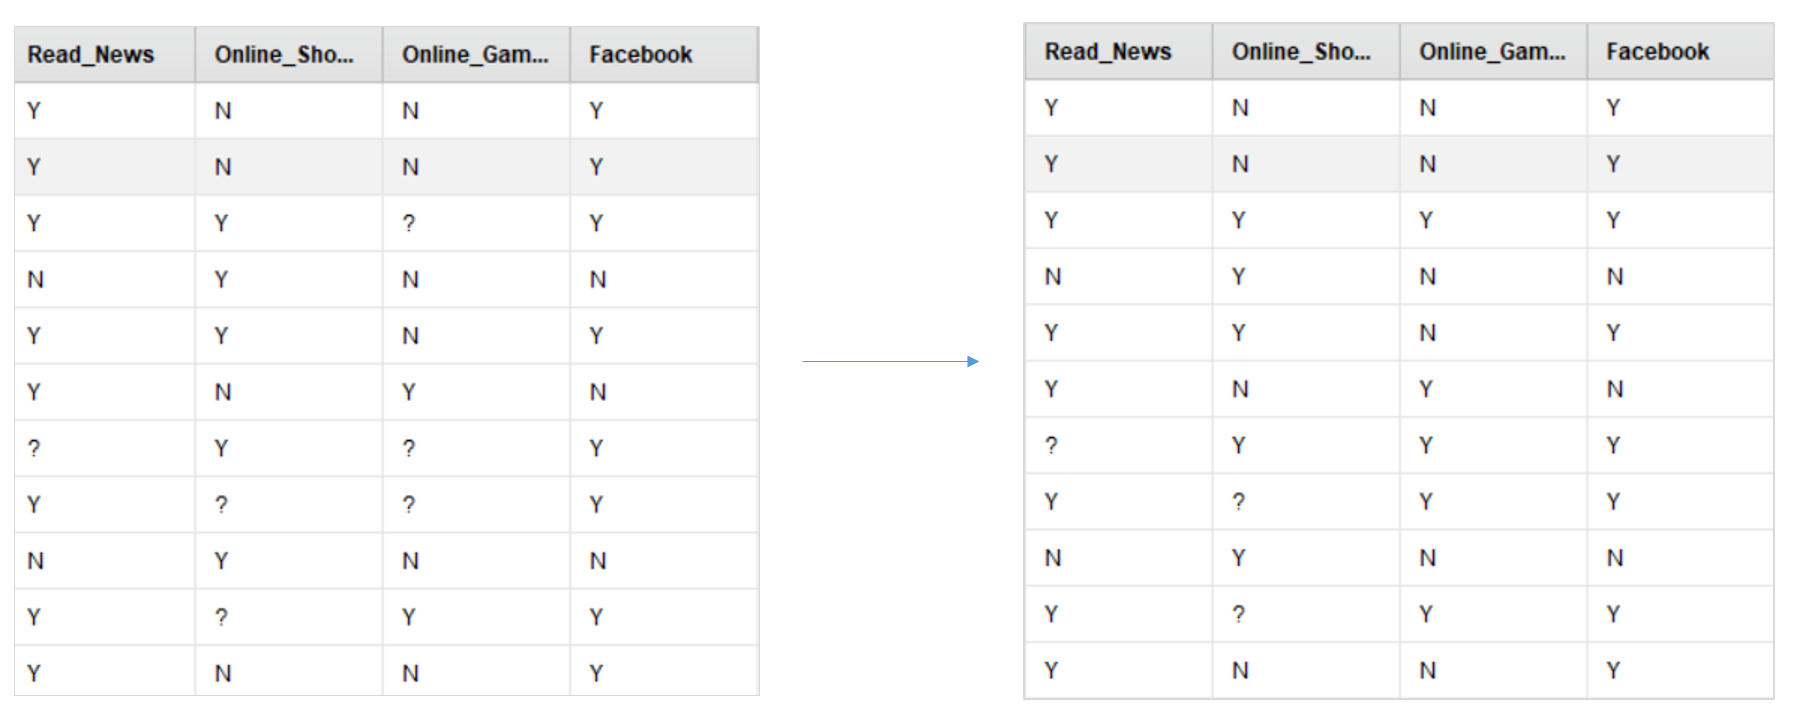
\includegraphics[width=0.6\textwidth]{1_beforeafter.png}
	\caption{Illustration of how missing values are filled.}
	\label{pl1}
\end{figure}

\subsection*{Example Filter}
Using \textit{Blending Filters} from the \textit{operators} section, we can apply an attribute \textit{type} filtering. Under operators, blending, examples, filters and then filter examples, right clock on the operator and change the condition class parameter to \textit{attribute-value-filter}. Change the parameter string to \textit{Online\_Shopping = .} and analyze the results.
\subsubsection*{Results}
Examples which their value of \textit{Online\_Shopping} is missing will be removed. Number of samples will be reduced from 11 to 9 examples. The missing values under \textit{Online\_Shopping} are gone.
\begin{figure}[!h]\centering
	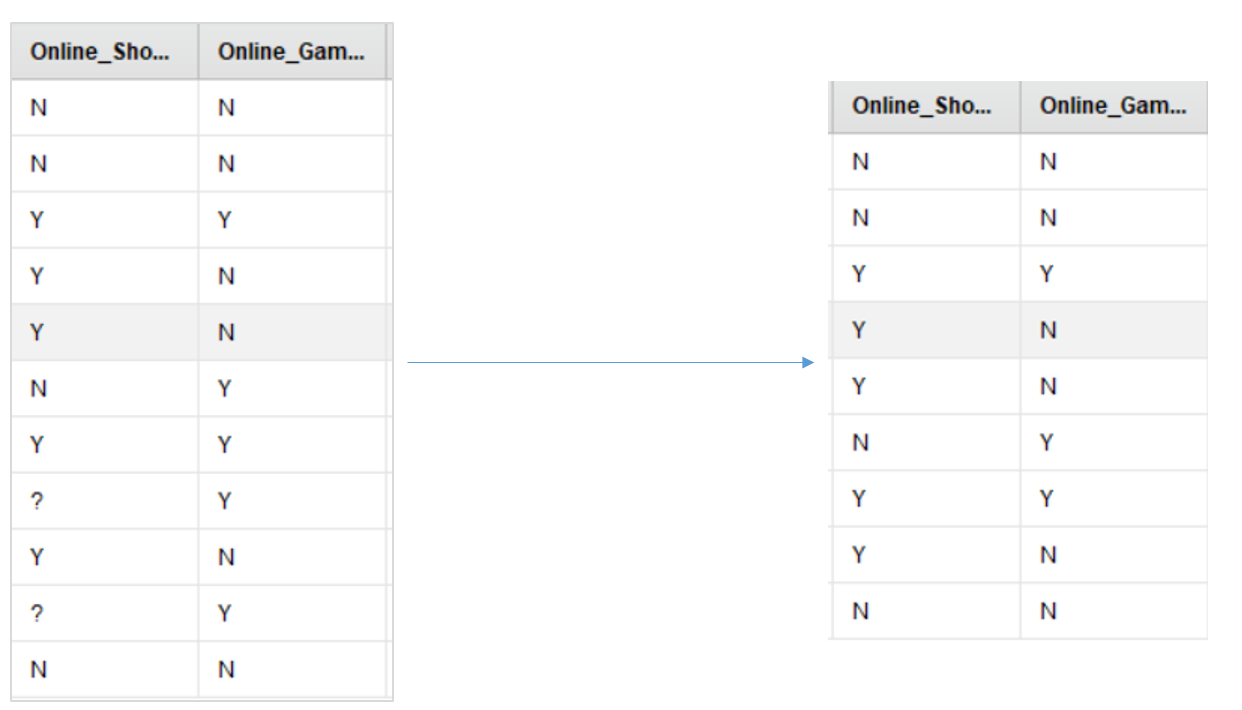
\includegraphics[width=0.6\textwidth]{2_beforeafter.png}
	\caption{Illustration of how samples with missing values are filtered.}
	\label{pl1}
\end{figure}

\subsection*{Sampling}
Use sampling to choose a subset of the examples. Initialize this operator to choose half of the dataset. Explain the parameters you choose and justify the results.
\subsubsection*{Results}
Out of 9 examples from the previous section, we'll set the sample size to 5. 

\subsection*{Store Results}
Choose the appropriate operator to store the result in \textit{.csv} or \textit{.xlsx} format.
\subsubsection*{Results}
Saved file is under \textit{preprocess} directory under \textit{src} folder. Figure 1.3 illustrates the final model.
\begin{figure}[!h]\centering
	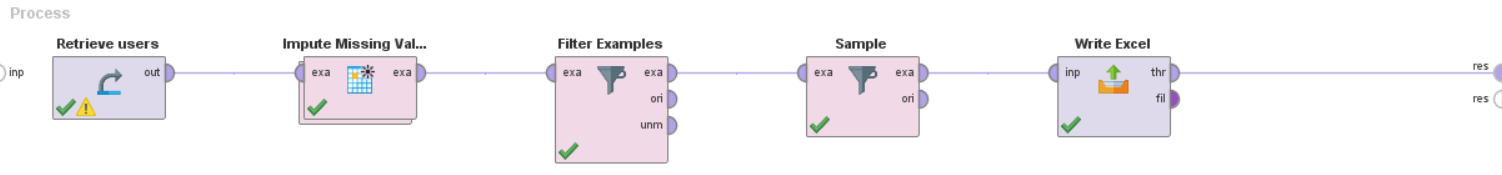
\includegraphics[width=0.8\textwidth]{3_preprocess_final.png}
	\caption{Illustration of final preprocessing model on \textit{users} dataset.}
	\label{pl1} 
\end{figure}

\section{Modeling a Decision Tree}
Use \textit{dt\_train} and \textit{dt\_score} datasets for this section.

\subsection*{Attributes Blending}
Under blending, attributes, names and roles, add \textit{set role} to the process. In both of the operators change \textit{attribute name} to \textit{User\_ID} and \textit{target role} to \textit{id}. Then connect training input to one and score input to another. Explain the purpose of this task?
\subsubsection*{Results}
The role of an Attribute describes how other Operators handle this Attribute. The default role is regular, other roles are classified as special. An ExampleSet can have many special Attributes, but each special role can only appear once. If a special role is assigned to more than one Attribute, all roles will be changed to regular except for the last Attribute. The different types of roles are explained below in the parameter section. An Attribute with the \textbf{id} role acts as an identifier for the Examples. It should be unique for all Examples. Different Blending Operators (Join, Union, Transpose, Pivot, ...) uses the id Attribute to perform their tasks.

\subsection*{Attributes Blending 2}
Add another \textit{set role} to the process. Change the attribute name to \textit{eReader\_Adoption}. Change the attribute type to \textit{label}. Explain the task.

\subsubsection*{Results}
This task provides a new column (which will be used for the test data) as a prediction column. Predicted labels will be filled in this column. This is also called the \textit{class} or \textit{target attribute}.

\subsection*{Model Training}
Under modeling, predictive, choose decision tree model. Run the model and explain the results.

\subsubsection*{Results}
Models starts to be trained after hitting the start process button. The learned decision tree can be found under  \textbf{Results}, \textbf{Graph} section. A part of this tree is given in figure 2.1.
\begin{figure}[!h]\centering
	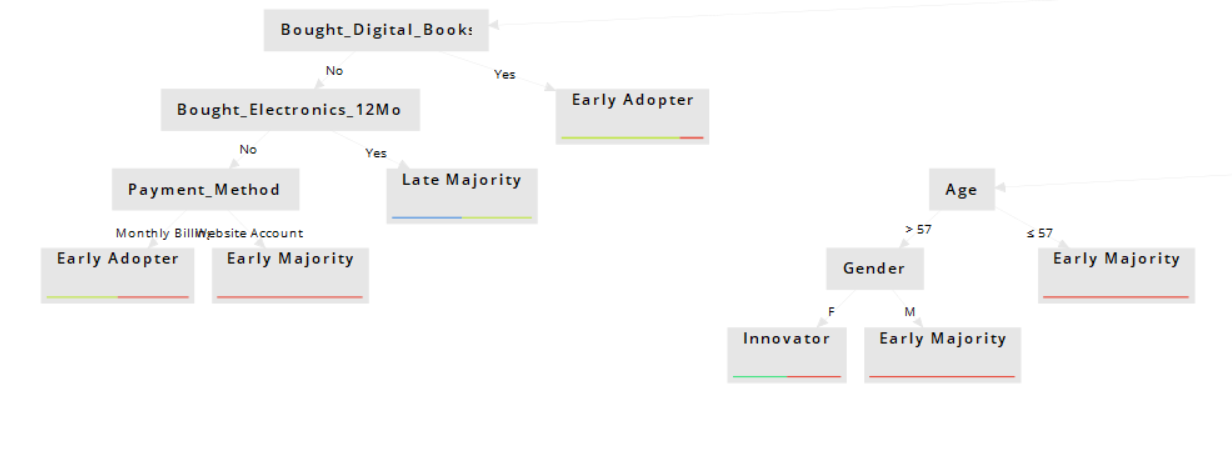
\includegraphics[width=0.8\textwidth]{4_dt_1.png}
	\caption{Illustration of a part of the Decision Tree model trained on the \textit{DT\_train} data.}
	\label{pl1} 
\end{figure}
Final model is provided in figure 2.2.
\begin{figure}[!h]\centering
	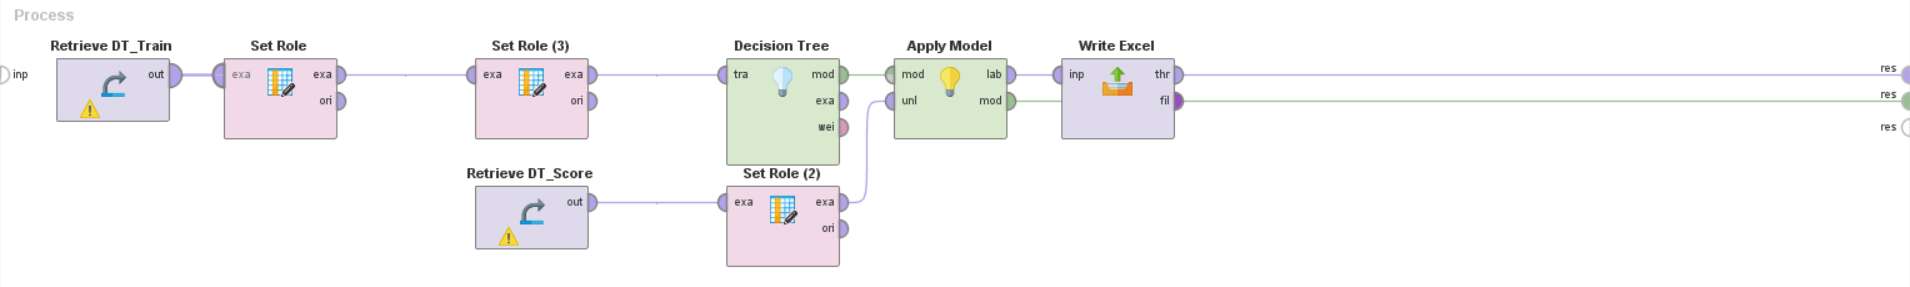
\includegraphics[width=0.8\textwidth]{4_dt_2.png}
	\caption{Illustration of the Decision Tree model trained on the \textit{DT\_train} data.}
	\label{pl1} 
\end{figure}
Prediction is classified into 4 classes. For each column (category), the confidence of the prediction. The label assigned to each sample will be the category with highest value of confidence. Figure 2.3 demonstrates a part of examples with their confidence results after applying the Decision Tree model.
\begin{figure}[!h]\centering
	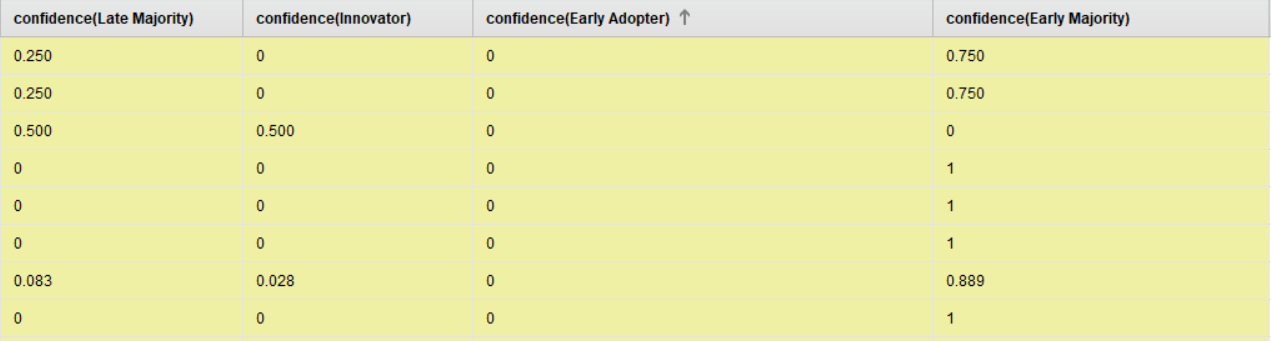
\includegraphics[width=0.8\textwidth]{4_dt_3.png}
	\caption{Demonstration of the Decision Tree prediction on the \textit{DT\_score} data.}
	\label{pl1} 
\end{figure}
Process data can be found under \textit{dt-results}.

\subsection*{Gini Indexing}
Change the decision tree criterion to \textit{gini-index}. Analyze the results.

\subsubsection*{Results}
Gini impurity is a measure of how often a randomly chosen element from the set would be incorrectly labeled if it was randomly labeled according to the distribution of labels in the subset.
\section{Naive Bayes Modeling}
Reform a model based on the Naive Bayes rule using the steps provided in the previous section. The goal attribute is \textit{Second Heart Attack}. Perform training and scoring the \textit{NB\_train} and \textit{NB\_score} data.
\subsection*{Results}
Prediction results is stored under \textit{src} directory in \textit{nb-results} folder.
\begin{figure}[!h]\centering
	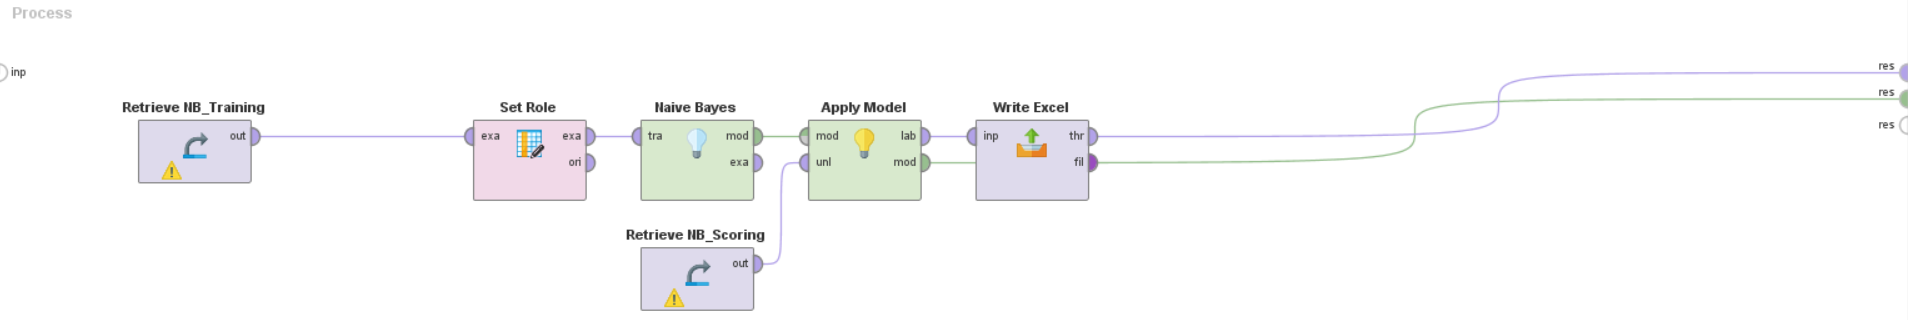
\includegraphics[width=0.8\textwidth]{1_nb_1.png}
	\caption{Illustration of Naive Bayes model trained on the \textit{NB-train} data.}
	\label{pl1} 
\end{figure}
\section{ROC Curve}
We'll use the \textit{NB-training} data for this section. From \textit{operations} section, find the \textit{Compare ROCs} operation. Add Decision Tree \& Naive Bayes (plus another random model for classification) in the ROC operator and complete the connections.
\begin{itemize}
	\item How are \textbf{ROC} curves plotted?
	
	To draw a ROC curve, only the true positive rate (TPR) and false positive rate (FPR) are needed (as functions of some classifier parameter). The TPR defines how many correct positive results occur among all positive samples available during the test. FPR, on the other hand, defines how many incorrect positive results occur among all negative samples available during the test.
	A ROC space is defined by FPR and TPR as x and y axes respectively, which depicts relative trade-offs between true positive (benefits) and false positive (costs). Since TPR is equivalent to sensitivity and FPR is equal to 1 − specificity, the ROC graph is sometimes called the sensitivity vs (1 − specificity) plot. Each prediction result or instance of a confusion matrix represents one point in the ROC space.
	The best possible prediction method would yield a point in the upper left corner or coordinate (0,1) of the ROC space, representing 100\% sensitivity (no false negatives) and 100\% specificity (no false positives). The (0,1) point is also called a perfect classification. A completely random guess would give a point along a diagonal line (the so-called line of no-discrimination) from the left bottom to the top right corners (regardless of the positive and negative base rates). An intuitive example of random guessing is a decision by flipping coins (heads or tails). As the size of the sample increases, a random classifier's ROC point migrates towards (0.5,0.5).
	The diagonal divides the ROC space. Points above the diagonal represent good classification results (better than random), points below the line poor results (worse than random). The ROC comparison results is given in the figure 4.1.
	
	\begin{figure}[!h]\centering
		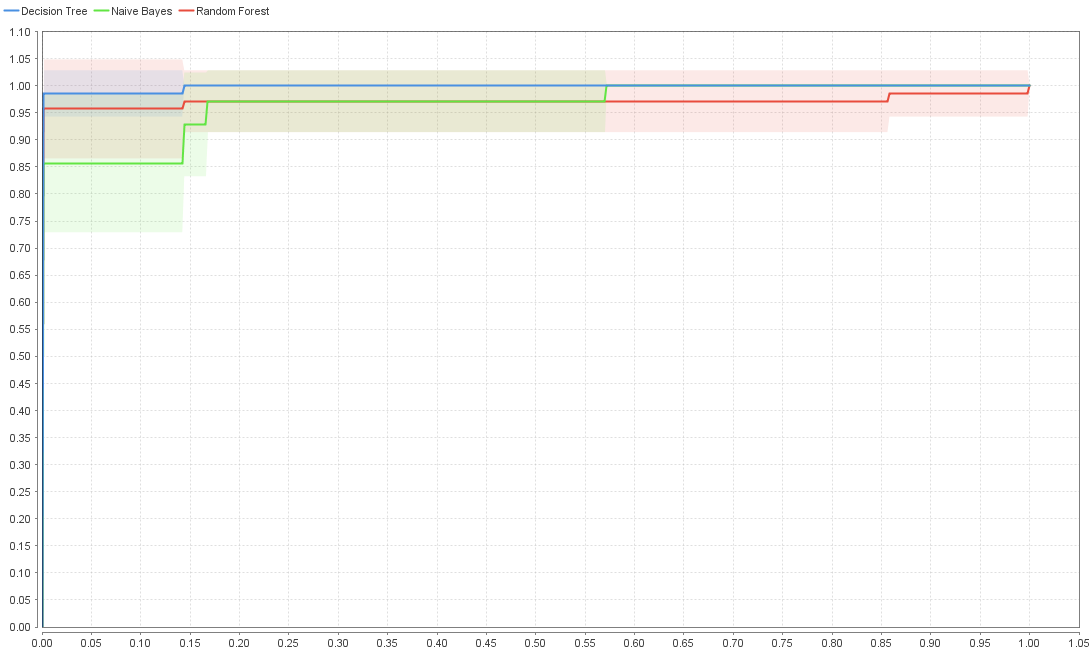
\includegraphics[width=0.7\textwidth]{roc.png}
		\caption{ROC Curve comparison for 3 models trained on \textit{NB-training} dataset.}
		\label{pl1} 
	\end{figure}


	\item What is the relationship between \textit{confidence} column and the ROC curve?
	
	A confidence interval gives an estimated range of values which is likely to include an unknown population parameter, the estimated range being calculated from a given set of sample data. (Definition taken from Valerie J. Easton and John H. McColl's Statistics Glossary v1.1). The higher AUC is (sometimes AUC is referred to as AUROC), the better model will be. Higher AUCs yields in more TPR and less FPR. Thus, each model with higher TPR and less FPR (practically smaller AUCs) will predict the TRUE labels as positive and FALSE labels as negative more often. This, simply means that the confidence (mathematical assurance for being correct) is higher for the models with higher AUCs.
	\item What is \textbf{AUC} and how is that analyzed?
	
	AUC is an abbrevation for area under the curve. It is used in classification analysis in order to determine which of the used models predicts the classes best. Please refer to the previous section for more information on \textbf{AUC}.
\end{itemize}
\end{document}